\documentclass[11pt]{standalone}

\usepackage{tikz}
\usetikzlibrary{positioning, arrows.meta, shapes.misc}
\usepackage{relsize}
\usepackage[detect-all]{siunitx}

\begin{document}
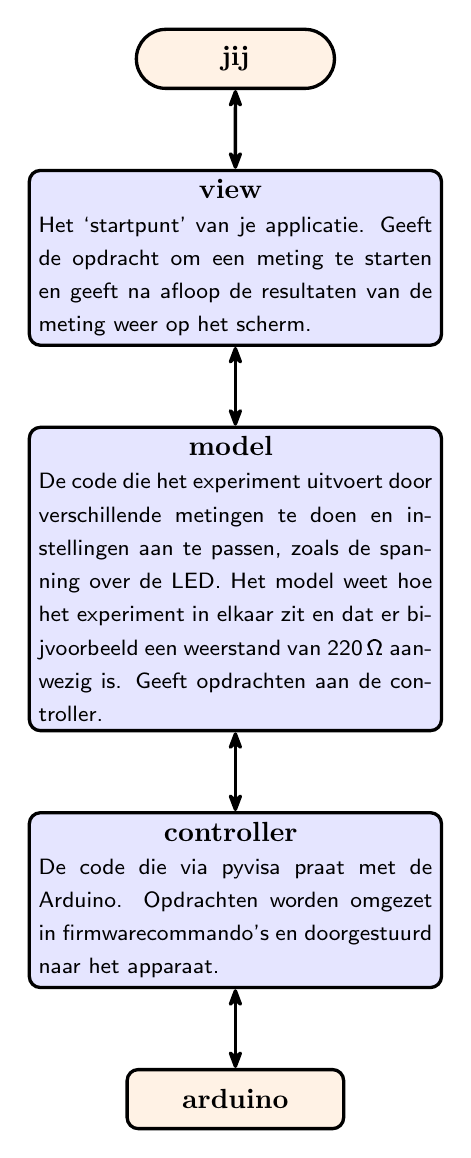
\begin{tikzpicture}[draw, very thick, every node/.style={draw, rounded corners, minimum width=2.75cm, minimum height=.75cm, node distance=1cm}, >={Stealth[round]}]
    \node[fill=orange!10, sharp corners, rounded rectangle] (user) {\textbf{jij}};
    \node[fill=blue!10] (view) [below=of user] {\parbox{5cm}{
            \hfill \textbf{view} \hfill{} \\
            \textsmaller{\sffamily
                Het `startpunt' van je applicatie. Geeft de opdracht om een meting te starten en geeft na afloop de resultaten van de meting weer op het scherm.
            }
        }
    };
    \node[fill=blue!10] (model) [below=of view] {\parbox{5cm}{
            \hfill \textbf{model} \hfill{} \\
            \textsmaller{\sffamily
                De code die het experiment uitvoert door verschillende metingen te doen en instellingen aan te passen, zoals de spanning over de LED. Het model weet hoe het experiment in elkaar zit en dat er bijvoorbeeld een weerstand van \qty{220}{\ohm} aanwezig is. Geeft opdrachten aan de controller.
            }
        }
    };
    \node[fill=blue!10] (controller) [below=of model] {\parbox{5cm}{
            \hfill \textbf{controller} \hfill{} \\
            \textsmaller{\sffamily
                De code die via pyvisa praat met de Arduino. Opdrachten worden omgezet in firmwarecommando's en doorgestuurd naar het apparaat.
            }
        }
    };
    % \node[fill=blue!10] (controller2) [below=of model,xshift=2cm] {controller};
    % \path (controller1) -- (controller2) node[midway,scale=2,lightgray,draw=none] {$\ldots$};
    \node[fill=orange!10] (dev) [below=of controller] {\textbf{arduino}};
    % \node[fill=orange!10] (dev2) [below=of controller2] {instrument};
    % \path (dev1) -- (dev2) node[midway,scale=2,lightgray,draw=none] {$\ldots$};

    \draw[<->] (user) -- (view);
    \draw[<->] (view) -- (model);
    \draw[<->] (model) -- (controller);
    % \draw[<->] (model) -- (controller2);
    \draw[<->] (controller) -- (dev);
    % \draw[<->] (controller2) -- (dev2);
\end{tikzpicture}
\end{document}